\documentclass[12pt]{standalone}
\usepackage{tikz}

\begin{document}

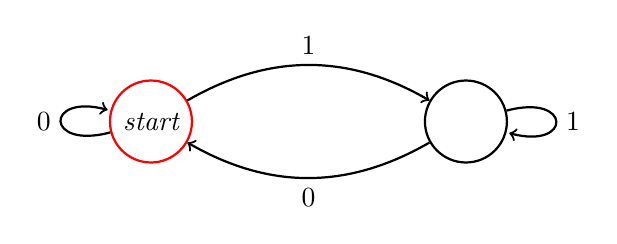
\begin{tikzpicture}[thick]
    \node[draw=red,fill=none,circle] (A) at (0,0) {$\textit{start}$};
    \node[draw=black,fill=none,circle] (B) at (4,0) {$\phantom{\textit{start}}$};
    \path (A) edge[->,bend left=30] node[pos=0.5,above] {$1$} (B);
    \path (B) edge[->,bend left=30] node[pos=0.5,below] {$0$} (A);
    \path (A) edge[->,loop left] node[left] {$0$} (A);
    \path (B) edge[->,loop right] node[right] {$1$} (B);
\end{tikzpicture}

\end{document}
